



%----------------------------------------------------------------------------------------

\newpage


%\section[Existing Models][Modèles existants]{Existing Models}{Modèles existants}
\section{Existing Models}{Modèles existants}

\label{sec:macrocoevolexplo}

%----------------------------------------------------------------------------------------


Nous proposons dans un premier temps d'introduire les modèles de co-évolution à l'échelle macroscopique en étudiant\comment[FL]{cela ne me semble pas un enchainement logique de verbes d'action} les résultats produits par des modèles existants, ce qui permettra également d'introduire les méthodes et indicateurs nécessaires à l'exploration du modèle, ainsi que d'appréhender les questionnements typiques liés à ce type de modèles. En particulier, nous procédons à une exploration systématique du modèle SimpopNet~\cite{schmitt2014modelisation}, l'une des rares initiatives pour modéliser la co-evolution au sein d'un système de villes.\comment[FL]{a notre connaissance}



%%%%%%%%%%%%%%%%%%%%%%%
\subsection{Context}{Contexte}


\bpar{
Which differences in produced knowledge can be observed, from the conceptual or thematic description of a model, to its mathematical formalisation, its implementation, its systematic exploration, up to its exploration in deep with the help of specific meta-heuristics ? Our postulate, that is a consequence of both our positioning (see \autoref{ch:positioning} on simulation) and experiments of which previously developed models are part, is that it is considerable, but furthermore of a \emph{qualitative} nature, in the sense that the nature of knowledge follows abrupt transitions during the advance of the investigation in this continuum. The SimpopNet model introduced by~\cite{schmitt2014modelisation}, which is to our knowledge the only co-evolution model in the perspective of the evolutive urban theory, is an example of such a preliminary approach that must be explored deeper, for example through systematic exploration.
}{
Quelle gain de connaissances obtenues peut s'observer, de la description conceptuelle ou thématique d'un modèle, à sa formalisation mathématique, son implémentation, son exploration systématique, jusqu'à son exploration approfondie à l'aide de meta-heuristiques spécifiques ?\comment[AB]{reformuler}\comment[FL]{c'est une question trop generique pour du chap 6} Notre postulat, qui découle à la fois de notre positionnement (voir \autoref{ch:positioning} sur la simulation) et d'expériences dont les modèles déroulés précédemment font partie, est que celui-ci est important, mais surtout de nature \emph{qualitative}\comment[AB]{{\_}}, c'est à dire que la nature même des connaissances subit des transitions abruptes lors de l'avancée de la démarche dans ce continuum. Le modèle SimpopNet introduit par~\cite{schmitt2014modelisation}, qui est à notre connaissance l'unique modèle de co-évolution dans une perspective de la théorie évolutive des villes, est un exemple d'une telle démarche préliminaire qui nécessite d'être creusée, par exemple par l'exploration systématique.\comment[AB]{me semble impropre fondé (?) comme terme (?) $\rightarrow$ de quoi ? des modèles, de leur comportement, de leur resultats ?}\comment[FL]{apport de ce paragraphe ?}
}


\paragraph{Model Description}{Description du Modèle}\comment[AB]{reformuler}

Nous reformulons brièvement le modèle, suivant les notations de la formulation du modèle d'interaction en~\ref{sec:interactiongibrat}, un certain nombre de paramètres et de processus se recoupant. Les villes croissent suivant la spécification de l'équation~\ref{eq:interactiongibrat:model},\comment[AB]{la rappeler} avec $r_0 = 0$, $w_G = \lambda^\beta \cdot N$ et $V_{ij} = \mu_j / d_{ij}^\beta$.\comment[FL]{rappeller l'interpretation thematique des notations} Le potentiel d'interaction ne dépend pas de la population de la ville d'origine, et le choix d'une fonction puissance permet de combiner un paramètre de décroissance $\lambda$ à un paramètre de forme $\beta$. Le réseau croît à chaque pas de temps par rupture topologique\comment[AB]{est-ce le meilleur terme ?}\comment[FL]{sens ?} : un couple de villes est choisi, la première selon les populations avec une hiérarchie $\gamma_N$ (c'est à dire avec une probabilité ${\mu_i}^{\gamma_N} / \sum_j {\mu_j}^{\gamma_N}$)\comment[FL]{estce vraiment necessaire d'utiliser des eq [our dire qu'une proba est proportionelle a la part de $\mu_i^{\gamma_N}$} et la seconde selon les potentiels d'interaction $\mu_i \mu_j / d_{ij}^\beta$ avec la même hiérarchie $\gamma_N$, puis un lien est créé si le réseau n'est pas assez efficace\comment[AB]{expliciter ce principe}\comment[FL]{sens efficace ?}, i.e. $d_{ij}/d^{(N)}_{ij}> \theta_N$. Les liens créés à une date $t$ ont une vitesse $v(t)$, qui dépendra des technologies de transport courantes. La planarisation\comment[FL]{sens ?} n'est effectuée que pour les liens de vitesse semblable. Pour étudier une version stylisée du modèle, nous considérons une configuration simplifiée telle que $v(t > 0) = v_0$ et $v(0) = 1$ (le modèle initial considère trois valeurs de la vitesse correspondant aux réalités des technologies de transport entre 1830 et 2000).\comment[FL]{alors presente peut etre seulement la version simplifiee}

\comment[FL]{pourquoi faire cette simplification ?}


\paragraph{Perspectives}{Perspectives}

Certains choix de modélisation ne sont pas en cohérence directe avec l'application qui en est faite : par exemple, une telle précision dans la paramétrisation des dates et des vitesses\comment[FL]{sens ? soit concret} en fait un modèle hybride, et devrait correspondre à une application sur une configuration spatiale réelle. Dans une configuration stylisée\comment[FL]{sens ?}, ces paramètres n'ont de sens que si l'on connait le comportement des dynamiques simulées, et en particulier le rôle de la configuration spatiale, c'est à dire la séparation entre effets structurels et effets conjoncturels. D'autre part, l'utilisation du modèle d'interaction sans le terme de Gibrat endogène serait difficilement adaptable pour une application du modèle sur données réelles vu les valeurs obtenues dans les études précédentes des modèles d'interaction, mais est bien cohérent dans un modèle stylisé, afin de comprendre les processus d'interaction de manière isolée, comme nous le ferons plus loin (mais en gardant à l'esprit que cette connaissance ne reflète pas nécessairement le comportement couplé, l'interaction entre les processus pouvant faire émerger de nouveaux comportements). La formulation du potentiel en $(\lambda / d_{ij})^\beta$ \comment[FL]{quest ce que $\lambda$ ?} implique que $\lambda$ capture à la fois le poids et la décroissance, mais permet moins de liberté\comment[FL]{sens ?} que la spécification que nous avons utilisé précédemment, et ne permet pas une interprétation en terme de flux limite\comment[FL]{sens ? c'est une vraie question}. L'introduction de l'effet tunnel \comment[FL]{c'est quoi, comment est-il introduit ?}dans le modèle, via les valeurs variables de $v(t)$ et le mécanisme de non-branchement\comment[AB]{ie de non-planarité par niveau de vitesse $\rightarrow$ preciser}, est exogène puisque spécifié dans les règles du modèle, contrairement au modèle d'interaction avec rétroaction des flux, dans lequel les variations de $w_N$ et $d_N$ doivent capturer un effet tunnel endogène\comment[FL]{c'est abscons}. L'introduction d'indicateurs spécifiques pour le mesurer serait une piste intéressante de développement, mais nous nous contentons de regarder ici la hiérarchie des centralités qui en est un bon indicateur.\comment[FL]{pourquoi devrions nous accepter cette affirmation ? effet tunnel et hierarchie cela semble n'avoir aucun lien.}[expliciter]



%%%%%%%%%%%%%%%%%%%%%%%
\subsection{Methodology}{Méthode}

\subsubsection{Spatial configuration}{Configuration spatiale}

Un aspect important de la compréhension des processus de co-évolution impliqués dans ce modèle est le rôle de la configuration spatiale initiale dans les motifs émergents observés. Nous appliquons pour cela la méthodologie développée en~\ref{sec:computation}, permettant d'étendre l'analyse de sensibilité d'un modèle à des méta-paramètres spatiaux.\comment[FL]{sens ?}

\paragraph{Synthetic configuration generation}{Génération de configuration synthétique}

Une système de villes synthétiques\comment[FL]{quest ce que cela signifie ?}, respectant au premier ordre de manière visuelle\comment[AB]{expliciter} les critères de l'état initial du modèle de base, est construit de la façon suivante (voir l'Appendice~\ref{app:sec:syntheticdata} pour la notion de données synthétiques, calibrées au premier et second ordre). Un nombre fixé de villes $N$ est réparti uniformément dans l'espace conditionnellement à une distance minimale entre chaque, et leur population est attribuée suivant une loi rang-taille dont les paramètres $P_{m}$ et $\alpha$ peuvent être ajustés (la distribution du modèle initial correspond à $\alpha\simeq 0.68$ avec $R^2=0.98$). Un squelette de réseau est créé par un algorithme de connexification\comment[FL]{?}, qui connecte les villes deux à deux par plus proche voisin\comment[FL]{c'est flou : mesure de distance ? espace euclidien ? pourquoi faire cela ?}, puis itérativement sélectionne un cluster aléatoirement et le connecte perpendiculairement au lien le plus proche hors du cluster. Le réseau est ensuite étoffé par la création de raccourcis locaux, par répétitions $n_s$ fois de la sélection aléatoire d'une ville selon les populations, et sa connexion à un voisin dans un rayon $r_s$ sous conditions de degré maximal $d_s$. Le réseau final est ensuite planarisé. Cette procédure crée des réseaux correspondant visuellement\comment[AB]{préciser criteres visuels} à l'initialisation du modèle, sachant qu'une instance du réseau ne permet pas de déterminer les distributions de paramètres topologiques sur lesquels une calibration plus fine pourrait être opérée.


\subsubsection{Indicators}{Indicateurs}

Un aspect crucial de l'étude des modèles de simulation est la définition d'indicateurs pertinents, surtout dans le cas de modèles synthétiques où il n'est pas possible de produire des sorties directement liées aux données par exemple. Des faits stylisés très généraux, comme vouloir produire une hiérarchie urbaine ou une hiérarchie de réseau, sont relativement limités. %Dans le cas de la hiérarchie particulièrement, les lois obtenues dévient d'une loi d'échelle et il est discutable d'utiliser uniquement la pente d'un ajustement brutal. % discutable, on fait justement un OLS brutal ; question pas si cruciale de plus ?
 De plus, la hiérarchie est produite mécaniquement par la majorité des modèles incluant des processus d'agrégation. Il faut donc des indicateurs plus élaborés pour comprendre les dynamiques du système.\comment[FL]{surtout il faut un questionnement, une grille de lecture qui rend les indicateurs necessaires. sinon c'est un pur jeu de l'esprit.}


Pour se concentrer sur la capacité du modèle à produire des trajectoires à la fois diverses et complexes, et par exemple sa capacité à produire des bifurcations qui se traduiraient par inversions de rang, ainsi que sa capacité à capturer différents aspects des dynamiques co-évolutives, nous proposons un jeu d'indicateurs, incluant par exemple des mesures de correlation retardée en écho aux régimes de causalité exhibés en~\ref{sec:causalityregimes}, ou une mesure de correlation en fonction de la distance, pour comprendre le rôle des interactions spatiales dans les couplages de trajectoires. Etant donné une variable $X_i(t)$ définie sur chacune des villes et dans le temps (qui pourra être la population ou des mesures de centralité par exemple), nous définissons les indicateurs :

\begin{itemize}
  \item Indicateurs basiques\comment[FL]{bof} : hiérarchie (pente du rang-taille) $\alpha (t)$, entropie $\varepsilon (t)$, statistiques descriptives $\hat{\Eb{X}} (t), \hat{\sigma} (t)$, de la distribution de $X_i$ dans le temps
  \item Corrélation de rang\comment[FL]{sens} entre l'instant initial et l'instant final, qui traduit la quantité de changement dans la hiérarchie lors de l'évolution du système : $\rho\left[X_i(t=0),X_i(t=t_f)\right]$
  \item Diversité des trajectoires, qui capture la diversité de forme des séries temporelles\comment[FL]{confusion possible avec forme urbaine et puis qu'est ce que cela signifie ?}, avec $\tilde{X}_i(t)\in \left[0;1\right]$ les trajectoires mises à l'échelle individuellement,
\[
\frac{2}{N\cdot(N-1)}\sum_{i<j} \left(\frac{1}{T}\int_{t} \left(\tilde{X}_i(t) - \tilde{X}_j(t)\right)^2 \right)^{\frac{1}{2}}
\]
\comment[AB]{expliciter cette variance $\rightarrow$ cf methode alternative Jasss}
\item Complexité moyenne des trajectoires, la ``complexité'' d'une trajectoire étant prise simplement dans notre cas par son nombre de points d'inflexion \comment[AB]{pas trivial a definir ca !}\comment[FL]{ah bon pourquoi est ce simple ?}
\item Corrélations en fonction de la distance, pour comprendre la manière dont l'effet de la distance est traduit au niveau macroscopique. Le profil de cette fonction, au regard des valeurs des paramètres de distance d'interaction inclus dans le modèle, traduira la tendance du modèle à faire émerger tel ou tel niveau d'interaction.
\[
\hat{\rho}_d\left[(X(\vec{x}_1,Y(\vec{x}_2))|||\vec{x}_1-\vec{x}_2||\sim d\right]
\]
\comment[AB]{pas clair}\comment[FL]{non comprehensible}
\item Corrélations retardées entre les variations, pour identifier des motifs de causalité entre les variables $X$ et $Y$. Les motifs $\hat{\rho}_{\tau}$ pour l'ensemble des variables sont à lire dans le sens des régimes potentiels, explorés en~\ref{sec:causalityregimes}.
\[
\hat{\rho}_{\tau}\left[\Delta X(t),\Delta Y(t-\tau)\right]
\]
\comment[AB]{pourquoi pas $\Delta Y(t)$ et $\Delta X (t+\tau)$ $\rightarrow$ ce deviendrait un modele avec anticipation plus que retard mais ca resterait $Y=f(X)$}
\end{itemize}

Ces indicateurs sont utilisés pour les populations $\mu_i(t)$\comment[FL]{pourquoi cela depend de t et ensuite non ?}, les centralités de proximité $c_i = \frac{1}{N-1}\sum_{i\neq j} \frac{1}{d_{ij}}$\comment[FL]{pourquoi cette mesure ?}, et les accessibilités $Z_i = \frac{1}{\sum_k \mu_k}\sum_{i\neq j} P_j \exp{\left(- d_{ij}/d_G\right)}$.



Nous introduisons de plus divers indicateurs de topologie du réseau, pour comprendre les formes finales produites par l'heuristique : diamètre, longueur moyenne de chemin, centralité de chemin moyenne et niveau de hiérarchie, performance moyenne, longueur totale.\comment[AB]{bien sur tous ces indicateurs sont definis quelque part.}




%%%%%%%%%%%%%%%%%%%%%%%
\subsection{Results}{Résultats}


\subsubsection{Experience plan}{Plan d'expérience}

Etant donne une configuration spatiale initiale (c'est a dire une valeur des meta-parametres), nous établissons les diagrammes de phase\comment[FL]{pourquoi souhaites-tu etablir des diagramme de phase ?} par l'exploration d'une grille de l'espace des paramètres. Le nombre de paramètres étant restreint et l'objectif étant un premier aperçu du comportement du modèle\comment[FL]{ce n'est pas une attente suffisante : cette exploration est necessairement au service d'un questionnement plus vaste}, nous ne faisons pas appel à des méthodes d'exploration plus élaborées. Les paramètres sont $(d_G,\gamma_G,\gamma_N,\theta_N,v_0)$ et les méta-paramètres $(N_S,\alpha_S,d_S,n_S)$. Nous explorons une grille de 16 configurations des meta-paramètres, 324 configurations et paramètres, et 30 réplications aléatoires, ce qui correspond à 155,520 simulations.\comment[AB]{realisees contretmt}\comment[FL]{tu ne dis pas comment tu as fait ces choix (cad dans quelle perspective)}



\subsubsection{Convergence}{Convergence}


Pour quantifier\comment[FL]{encore un debut de par enigmatique} la variabilité d'un indicateur $X$ par rapport à la stochasticité, nous utilisons une mesure de type ratio de Sharpe\comment[FL]{source ?}, donnée par $v\left[X\right] = \hat{\Eb{X}}/\hat{\sigma\left[X\right]}$ avec les estimateurs basiques pour l'espérance et l'écart-type. Sur l'ensemble des exécutions\comment[FL]{replications ? vocab a harmoniser avec la literature}, on obtient sur l'ensemble des indicateurs donnés précédemment, une médiane\comment[AB]{mediane ou moyenne ?} estimée sur l'ensemble\comment[AB]{repet ensemble} des valeurs des paramètres, pour le ratio estimé au sein des réplications, qui prend une valeur minimale de $3.94$, pour la moyenne de l'accessibilité à l'instant final, ce qui témoigne d'une faible variabilité stochastique. On peut de plus utiliser cette valeur pour estimer le niveau de convergence : elle correspond à un intervalle de confiance à 95\% autour de la moyenne de taille relative $0.18$ (sous hypothèse de distribution normale de la moyenne), c'est à dire une bonne convergence.\comment[FL]{pourquoi voudrait-on quantifier une telle chose ?}


%On s'en sert egalement pour comparer la variabilité a la stochasticité a celle par rapport aux paramètres ou meta-paramètres, par exemple en calculant $v\left[X|\vec{\alpha}_1\right]/v\left[X|\vec{\alpha}_2\right]$ pour deux valeurs différentes des paramètres. \comment[JR]{pas besoin, on utilise la methode de spacematters, pour coherence. pas exactement pareil toutefois.}

% values of summaries for Sharpe ratios
%
%[1] "accessibilityEntropies95"
%    Min.  1st Qu.   Median     Mean  3rd Qu.     Max.     NA's 
%   4.038   13.704   35.392   95.136   93.556 4064.812        9 
%[1] "accessibilityHierarchies_alpha95"
%   Min. 1st Qu.  Median    Mean 3rd Qu.    Max.    NA's 
%  1.538   6.330   8.912   8.810  11.090  92.960       9 
%[1] "accessibilitySummaries_mean95"
%    Min.  1st Qu.   Median     Mean  3rd Qu.     Max.     NA's 
%  0.5106   2.8426   3.9498   5.2793   6.0301 155.6903        9 
%[1] "closenessEntropies95"
%   Min. 1st Qu.  Median    Mean 3rd Qu.    Max.    NA's 
%  11.25   39.70   85.78  106.72  154.51  677.88       9 
%[1] "closenessHierarchies_alpha95"
%   Min. 1st Qu.  Median    Mean 3rd Qu.    Max.    NA's 
%  2.429   5.107   6.933   7.803   9.930  48.226       9 
%[1] "closenessSummaries_mean95"
%   Min. 1st Qu.  Median    Mean 3rd Qu.    Max.    NA's 
%  1.391   3.488   5.753   6.018   7.901  39.855       9 
%[1] "populationEntropies95"
%    Min.  1st Qu.   Median     Mean  3rd Qu.     Max.     NA's 
%       3       51      953   646296    17776 35961483        9 
%[1] "populationHierarchies_alpha95"
%   Min. 1st Qu.  Median    Mean 3rd Qu.    Max.    NA's 
%      5      42     906  135579    3672 5328192       9 
%[1] "populationSummaries_mean95"
%    Min.  1st Qu.   Median     Mean  3rd Qu.     Max.     NA's 
%       1       17      382   229768     6319 11448551        9 
%[1] "complexityAccessibility"
%   Min. 1st Qu.  Median    Mean 3rd Qu.    Max.    NA's 
%     NA      NA      NA     NaN      NA      NA    2544 
%[1] "complexityCloseness"
%    Min.  1st Qu.   Median     Mean  3rd Qu.     Max.     NA's 
%  0.7363   4.6781  14.1490  16.0315  24.4733 221.7233        9 
%[1] "complexityPop"
%   Min. 1st Qu.  Median    Mean 3rd Qu.    Max.    NA's 
%     NA      NA      NA     NaN      NA      NA    2544 
%[1] "diversityAccessibility"
%    Min.  1st Qu.   Median     Mean  3rd Qu.     Max.     NA's 
%  0.6063   2.8002   6.2182   6.3092   9.0482 171.3062        9 
%[1] "diversityCloseness"
%   Min. 1st Qu.  Median    Mean 3rd Qu.    Max.    NA's 
% 0.8169  3.3100  7.3997  7.1288  9.5683 32.9526       9 
%[1] "diversityPop"
%   Min. 1st Qu.  Median    Mean 3rd Qu.    Max.    NA's 
%  1.058   4.089   7.481   8.001  10.858 115.732       9 





\subsubsection{Sensitivity to space}{Sensibilité à l'espace}

La table~\ref{tab:macrocoevolexplo:spacematters}\comment[AB]{pas vraiment exploitee} donne les valeurs de $\tilde{d}$\comment[AB]{definir} pour 16 configurations des méta-paramètres, par rapport à une configuration de référence arbitraire (première colonne). La hiérarchie au sein du système de villes initial est le plus fort déterminant, puisque l'ensemble des configurations avec $\alpha_S = 1.5$ donne des valeurs supérieures à 1.7, ce qui témoigne d'une très forte sensibilité relative à cette hiérarchie. Ensuite, le nombre de villes joue un rôle secondaire non-négligeable, donnant les plus forts effets de l'espace. Ainsi, il est crucial de garder à l'esprit ce rôle de la configuration initiale\comment[FL]{oui et a mon avis c'est un point a mettre en evidence un peu partout dans ta these} lors de l'analyse des diagrammes de phase. Pour rester dans l'esprit du modèle initialement proposé, nous commenterons toutefois un diagramme de phase pour une configuration spatiale donnée. L'étude du modèle étendu avec intégration des meta-paramètres auquel il est sensible comme paramètres à part entière est hors de portée de cette analyse auxiliaire. \comment[AB]{pas clair}\comment[FL]{tu peux parler de ca de facon plus simple}


%%%%%%%%%%%%%
\begin{table}[!ht]
\caption[Sensibility to space][Sensibilité à l'espace]{}{\textbf{Sensibilité à l'espace du modèle SimpopNet.} Chaque colonne correspond à une instance du diagramme de phase, pour laquelle les meta-paramètres sont donnés, ainsi que la distance relative à un diagramme de référence arbitraire.\comment[FL]{auest ce qui est input/output?}\label{tab:macrocoevolexplo:spacematters}}
\begin{tabular}{|l|l|l|l|l|l|l|l|l|l|l|l|l|l|l|l|l|}
\hline
$N_S$ & 40 & 40 & 40 & 40 & 40 & 40 & 40 & 40 & 80 & 80 & 80 & 80 & 80 & 80 & 80 & 80\\
$\alpha_S$ & 0.5 & 0.5 & 0.5 & 0.5 & 1.5 & 1.5 & 1.5 & 1.5 & 0.5 & 0.5 & 0.5 & 0.5 & 1.5 & 1.5 & 1.5 & 1.5\\
$d_S$ & 5 & 5 & 10 & 10 & 5 & 5 & 10 & 10 & 5 & 5 & 10 & 10 & 5 & 5 & 10 & 10\\
$n_S$ & 10 & 30 & 10 & 30 & 10 & 30 & 10 & 30 & 10 & 30 & 10 & 30 & 10 & 30 & 10 & 30\\
$\tilde{d}$ & 0 & 0.05 & 0.26 & 0.21 & 1.79 & 1.80 & 1.79 & 1.72 & 0.44 & 0.36 & 0.42 & 0.42 & 2.25 & 2.23 & 2.24 & 2.21\\\hline
\end{tabular}
\end{table}
%%%%%%%%%%%%%



\subsubsection{Patterns}{Motifs}


La Fig.~\ref{fig:macrocoevolexplo:behavior} rend compte du comportement du modèle selon les divers indicateurs donnés ci-dessus. Nous commentons une configuration spatiale particulière\comment[AB]{la qualifier}, donnée par les méta-paramètres $N_S=80,\alpha_S=0.5,d_S=10,n_S=30$.\comment[FL]{pourquoi ces choix ?} Les graphes complets sont disponibles en Appendice~\ref{sec:app:}. Les valeurs prises par l'entropie\comment[AB]{ou ca ?} pour les centralités, en fonction du temps, pour $\gamma_N = 2.5$ et $v_0 = 110$, exhibent différents régimes en fonction de $d_G$ et $\gamma_G$. Une faible hiérarchie conduit à une entropie se stabilisant dans le temps, correspondant à une certaine uniformisation des distances. Au contraire, une forte hiérarchie produit un régime avec un minimum, puis une augmentation des disparités dans le temps. Ce régime est illustré en premier panel de la Fig.~\ref{fig:macrocoevolexplo:behavior}.


Cette variété de comportements se retrouve avec la corrélation de rang $\rho_R$, que nous montrons ici pour la variable de population, en fonction de $d_G$. Celle-ci est peu sensible à $\theta_N$ et $\gamma_N$, mais varie fortement en fonction de $d_G$ et $\gamma_G$ : des interactions à plus longue distance induisent systématiquement un plus grand nombre d'inversions de hiérarchie\comment[FL]{expliciter plus clairement ce que cela signifie} (qui est la notion capturée par cet indicateur), et celles-ci peuvent avoir lieu quand la hiérarchie du potentiel gravitaire est faible.\comment[FL]{B} En résumé, l'augmentation de la portée des interactions complexifie\comment[FL]{?} la trajectoire du système de villes, tandis que l'augmentation de leur hiérarchie la simplifiera.\comment[FL]{alors est ce que la hierarchie est un input ou bien un output dans ce modele ?}


\comment[AB]{Aerer}

\comment[AB]{faire des ponts avec le thematique}

Concernant l'effet de la distance sur les corrélations entre variables, c'est à dire l'évolution de $\rho_d$, il est intéressant de noter que l'augmentation de $d_G$ diminue systématiquement les niveaux de correlation, ce qui correspond à la complexification mise en valeur précédemment. Comme attendu, $\rho_d\left[d\right]$ a un comportement décroissant\comment[FL]{md}, et des valeurs non-nulles pour la correlation entre population et centralité pour une forte hiérarchie $\gamma_G$, ce qui montre que les régimes d'adaptation simultanée sont rares dans ce modèle. De même, les régimes de causalité au sens de~\ref{sec:causalityregimes}, sont relativement pauvres : la population est systématiquement causée par la centralité, mais il n'existe pas de régime où l'on observe le contraire. On est dans la logique d'un effet de renforcement de la hiérarchie par la centralité, mais pas dans une configuration avec causalités circulaires, et donc pas dans une co-évolution à proprement parler comme nous l'avons défini.\comment[FL]{effectivement il est important d'avoir clairement defini ce concept \ldots ce qui n'est pas encore le cas ici} Cette exploration brève nous permet d'affirmer que ce modèle capture des trajectoires urbaines d'une certaine complexité, mais qu'il ne reproduit pas des régimes de co-évolution mais de co-adaptation. Par la suite, nous explorerons dans le même esprit une extension co-évolutive du modèle d'interaction développé en~\ref{sec:interactiongibrat}, et chercherons à établir dans quelle mesure il est capable de capturer des dynamiques co-évolutives.



%%%%%%%%%%%%%%%%
\begin{figure}
	%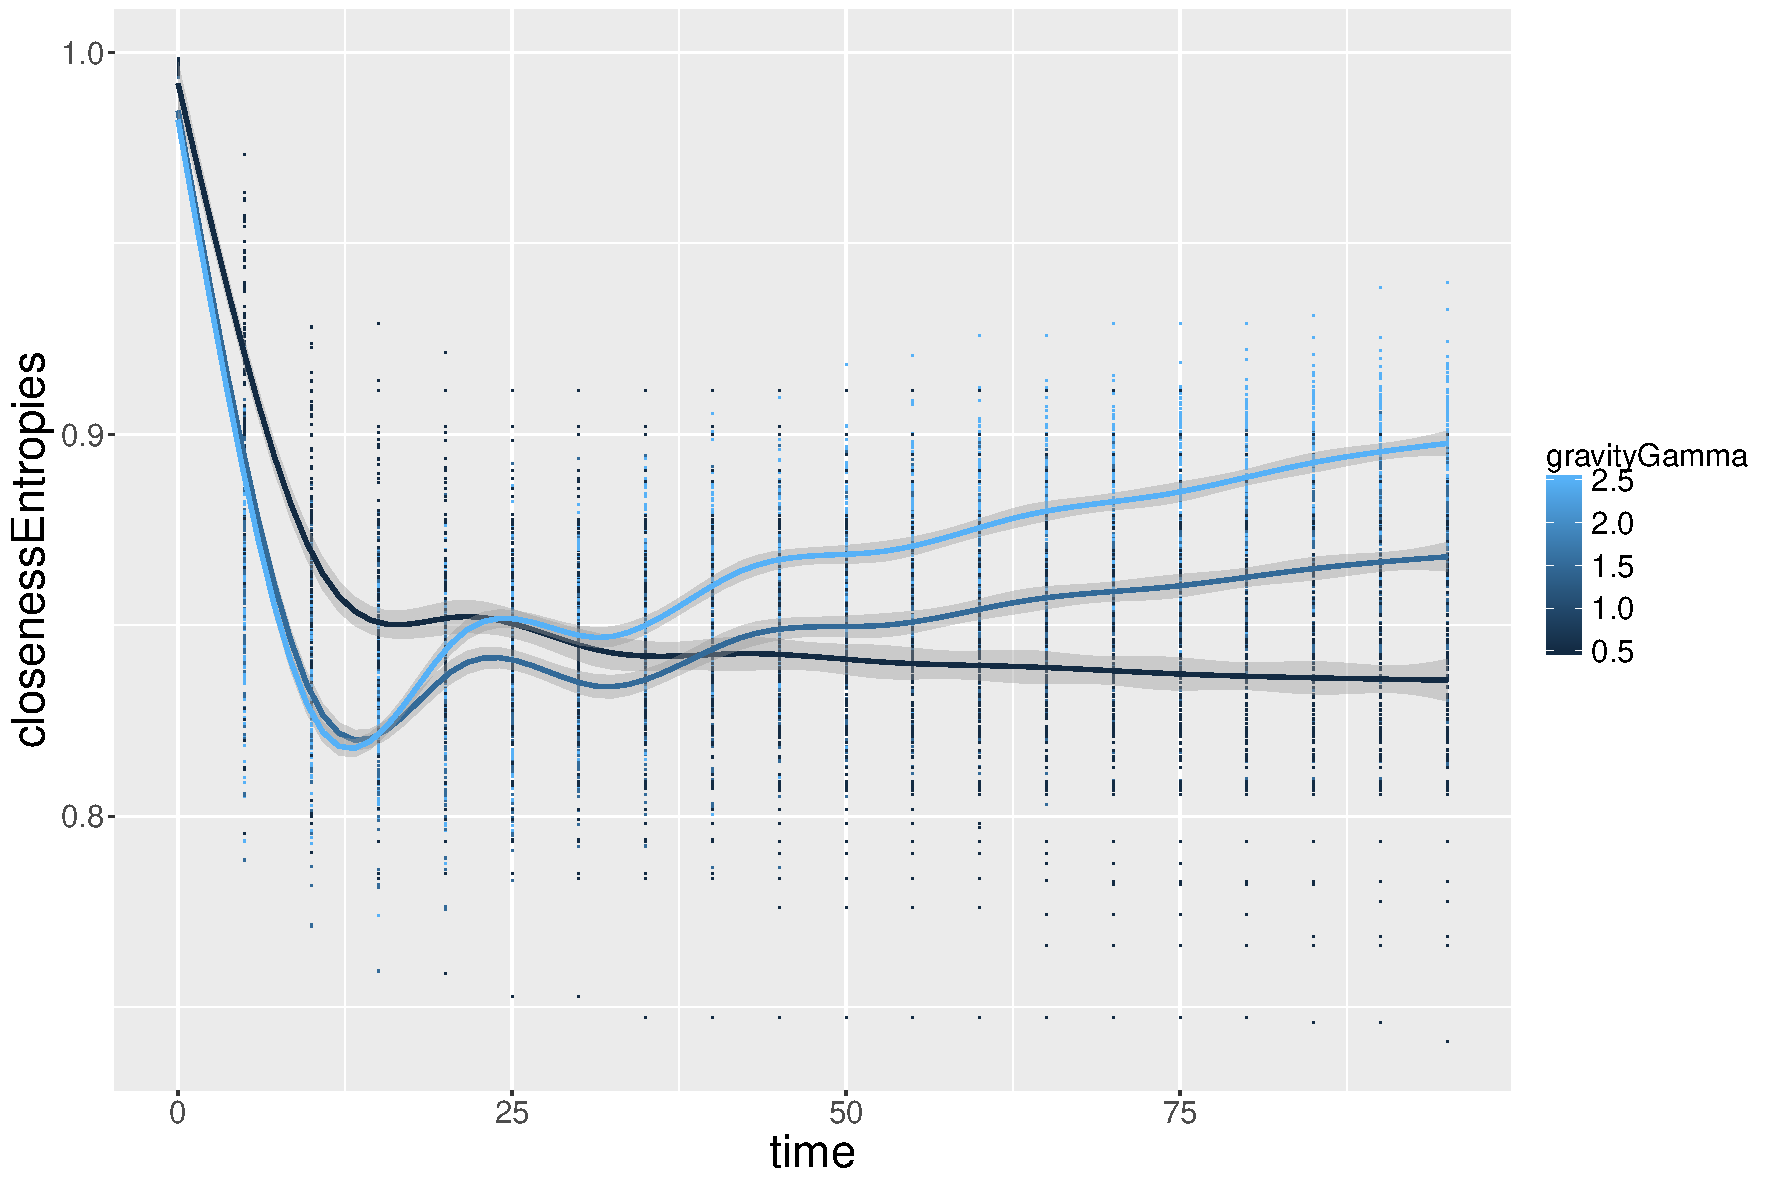
\includegraphics[width=0.48\linewidth]{Figures/MacroCoEvolExplo/closenessEntropies_networkGamma2.5_networkSpeed110_gravityDecay0.016_networkThreshold11.pdf}
	%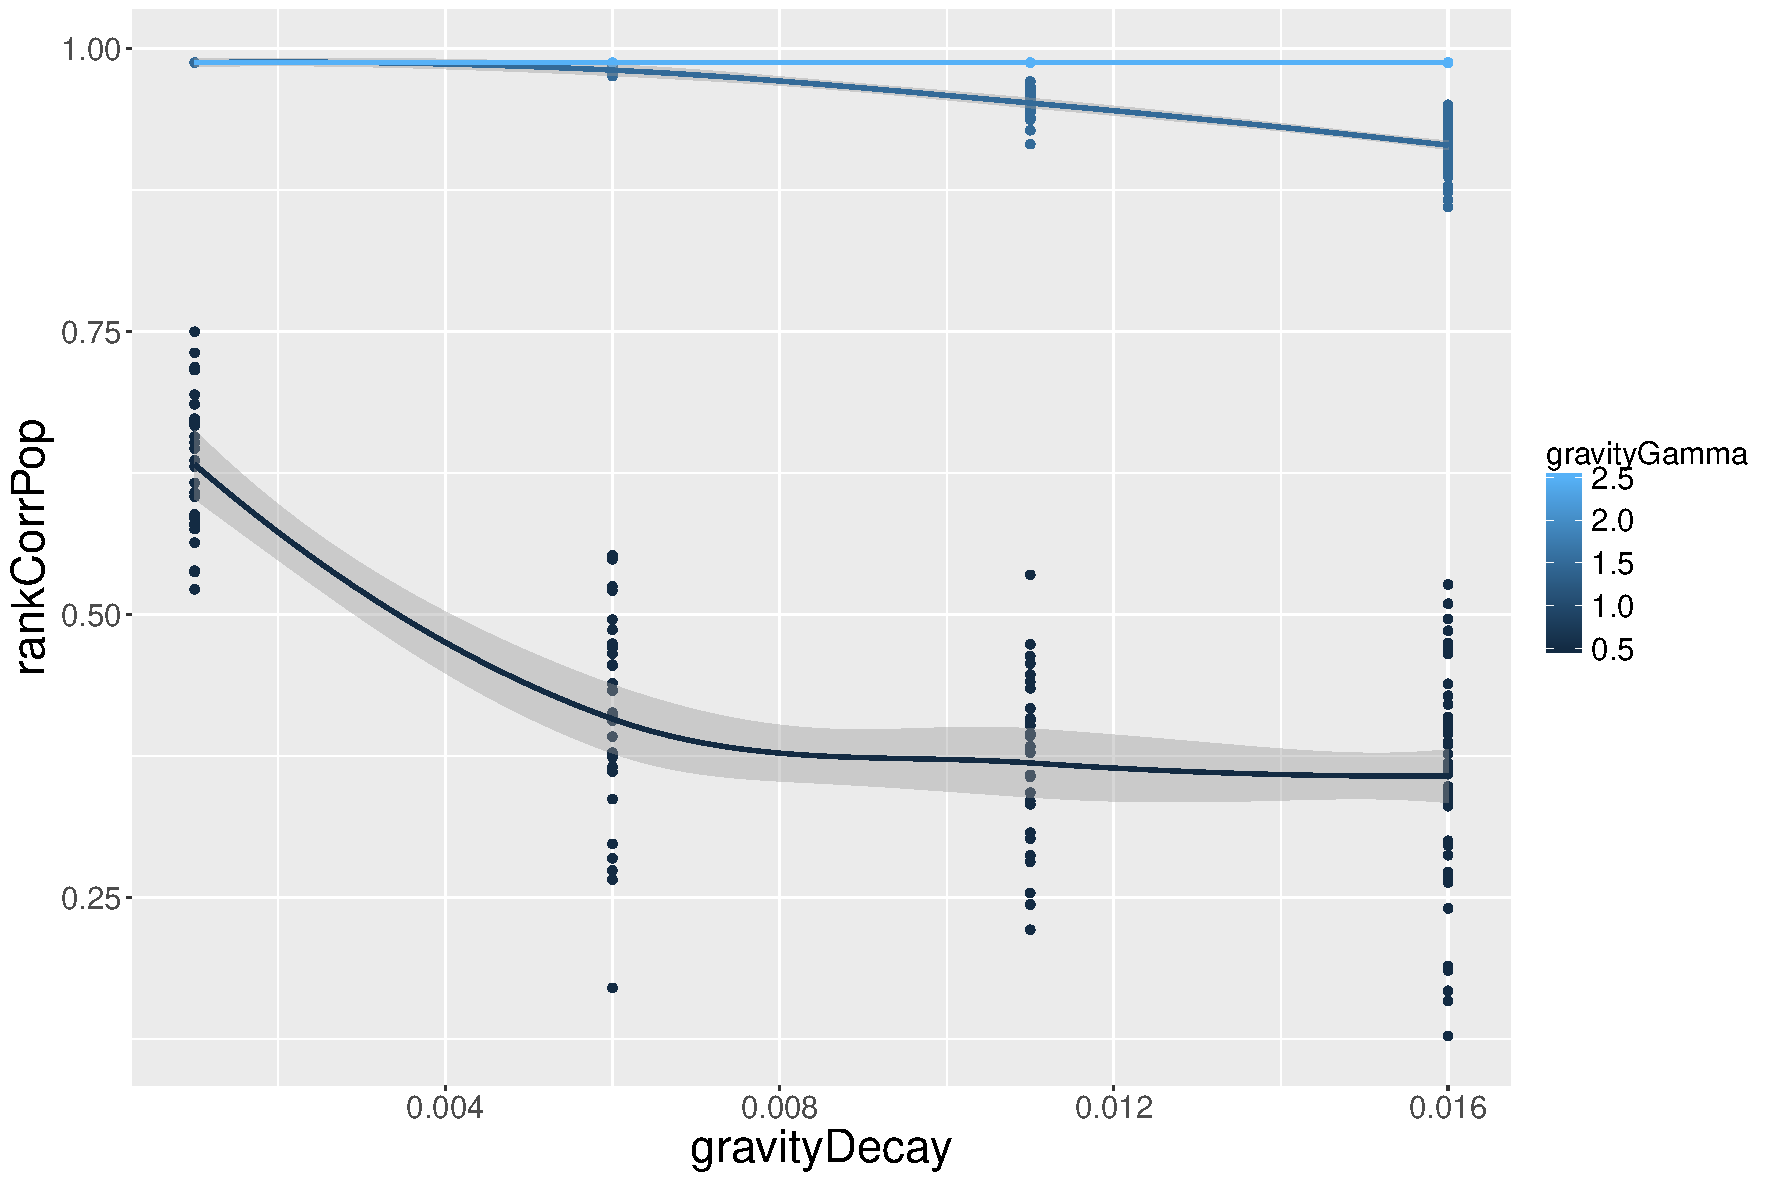
\includegraphics[width=0.48\linewidth]{Figures/MacroCoEvolExplo/rankCorrPop_networkSpeed110_networkThreshold11_networkGamma2.5.pdf}\\
	%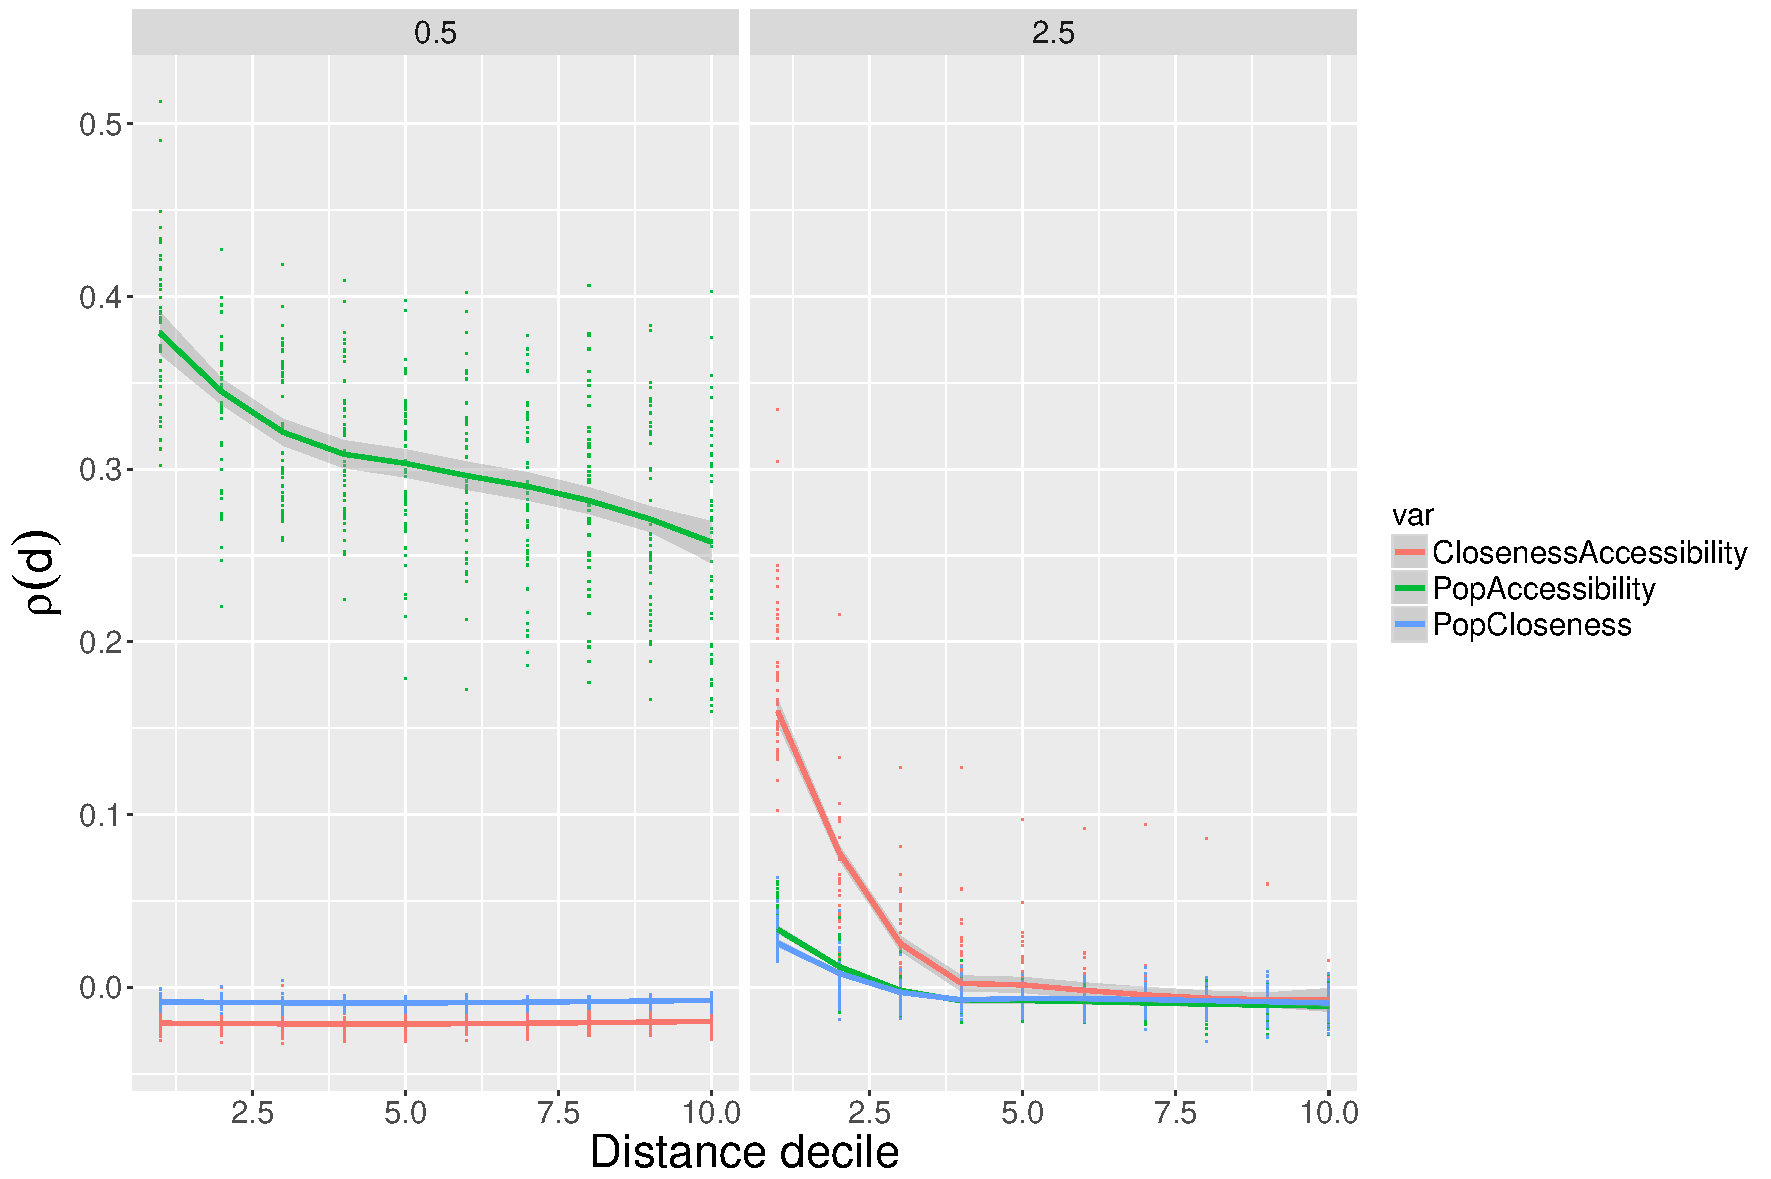
\includegraphics[width=0.48\linewidth]{Figures/MacroCoEvolExplo/distcorrs_networkGamma2.5_networkSpeed110_gravityDecay0.016_networkThreshold11.pdf}
	%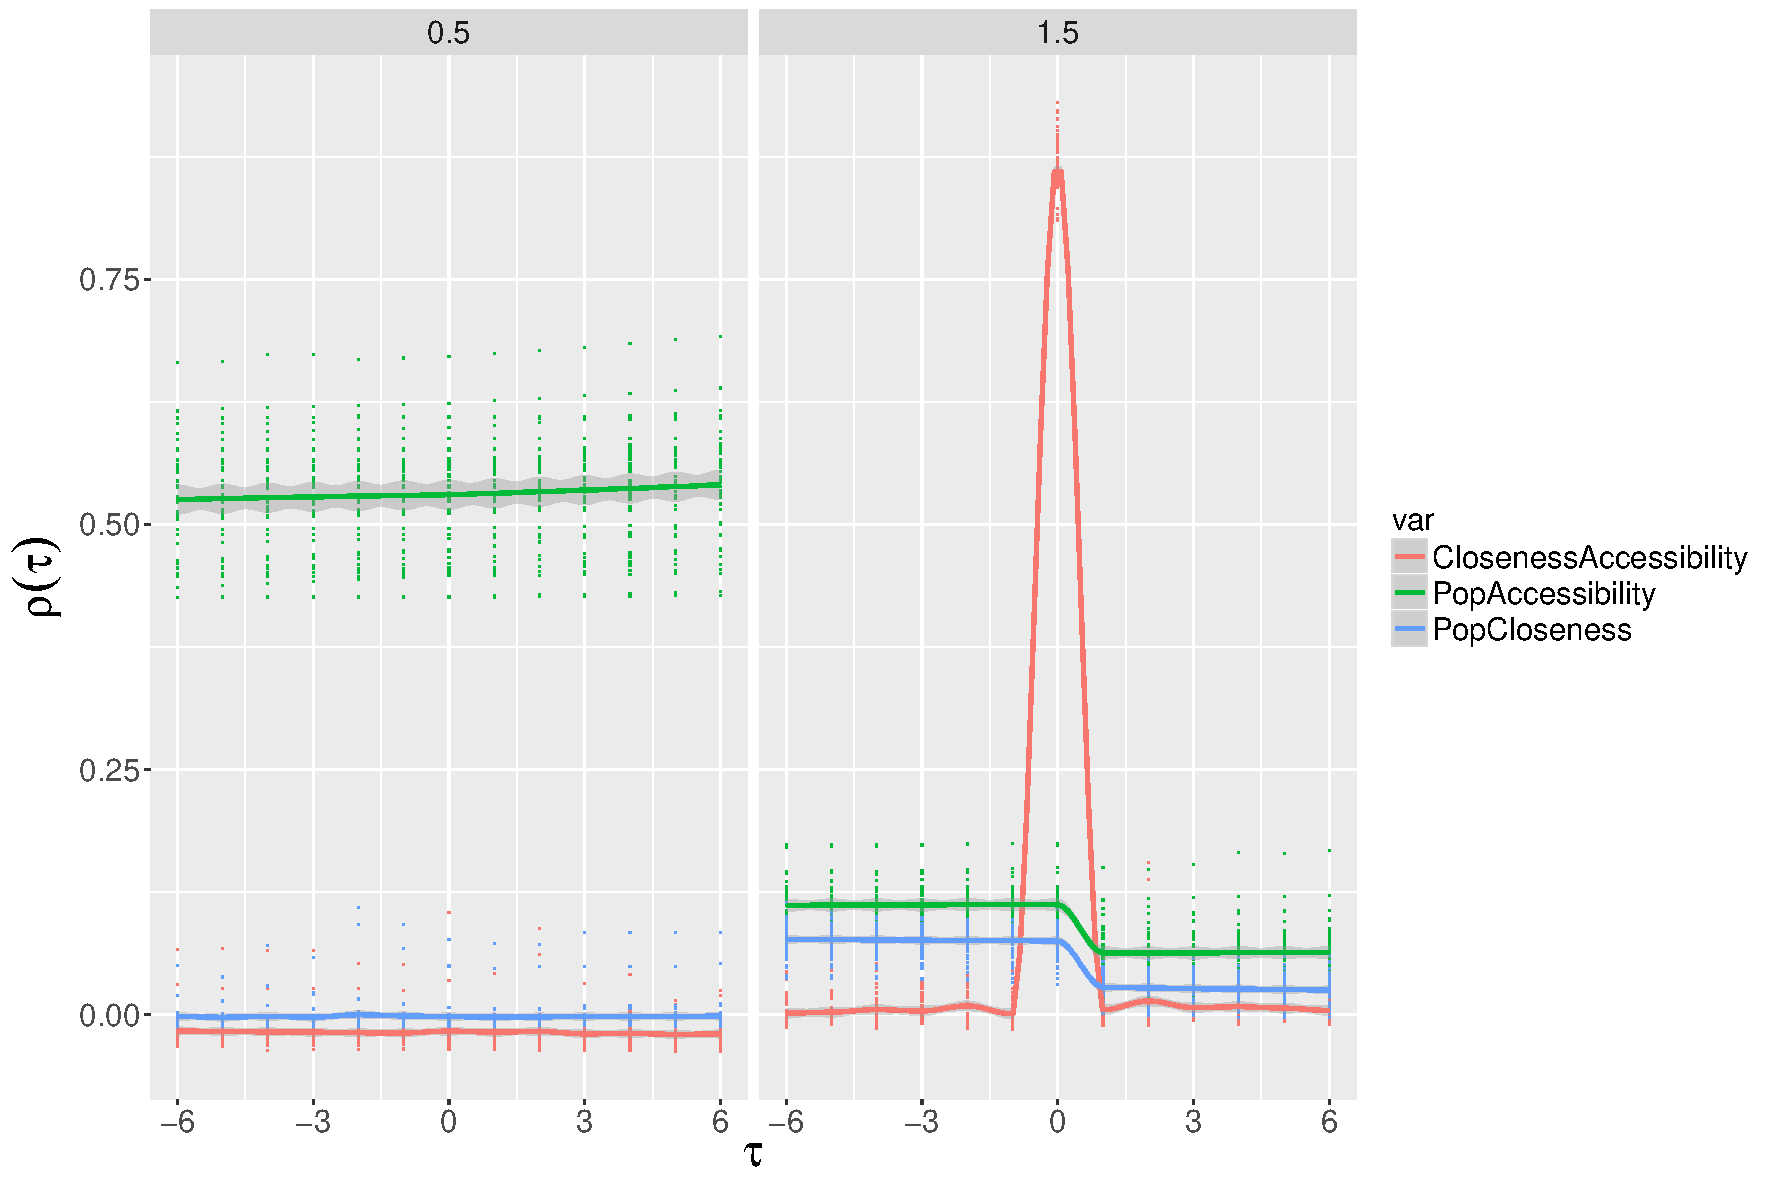
\includegraphics[width=0.48\linewidth]{Figures/MacroCoEvolExplo/laggedcorrs_networkGamma2.5_networkSpeed10_gravityDecay0.016_networkThreshold21.pdf}
	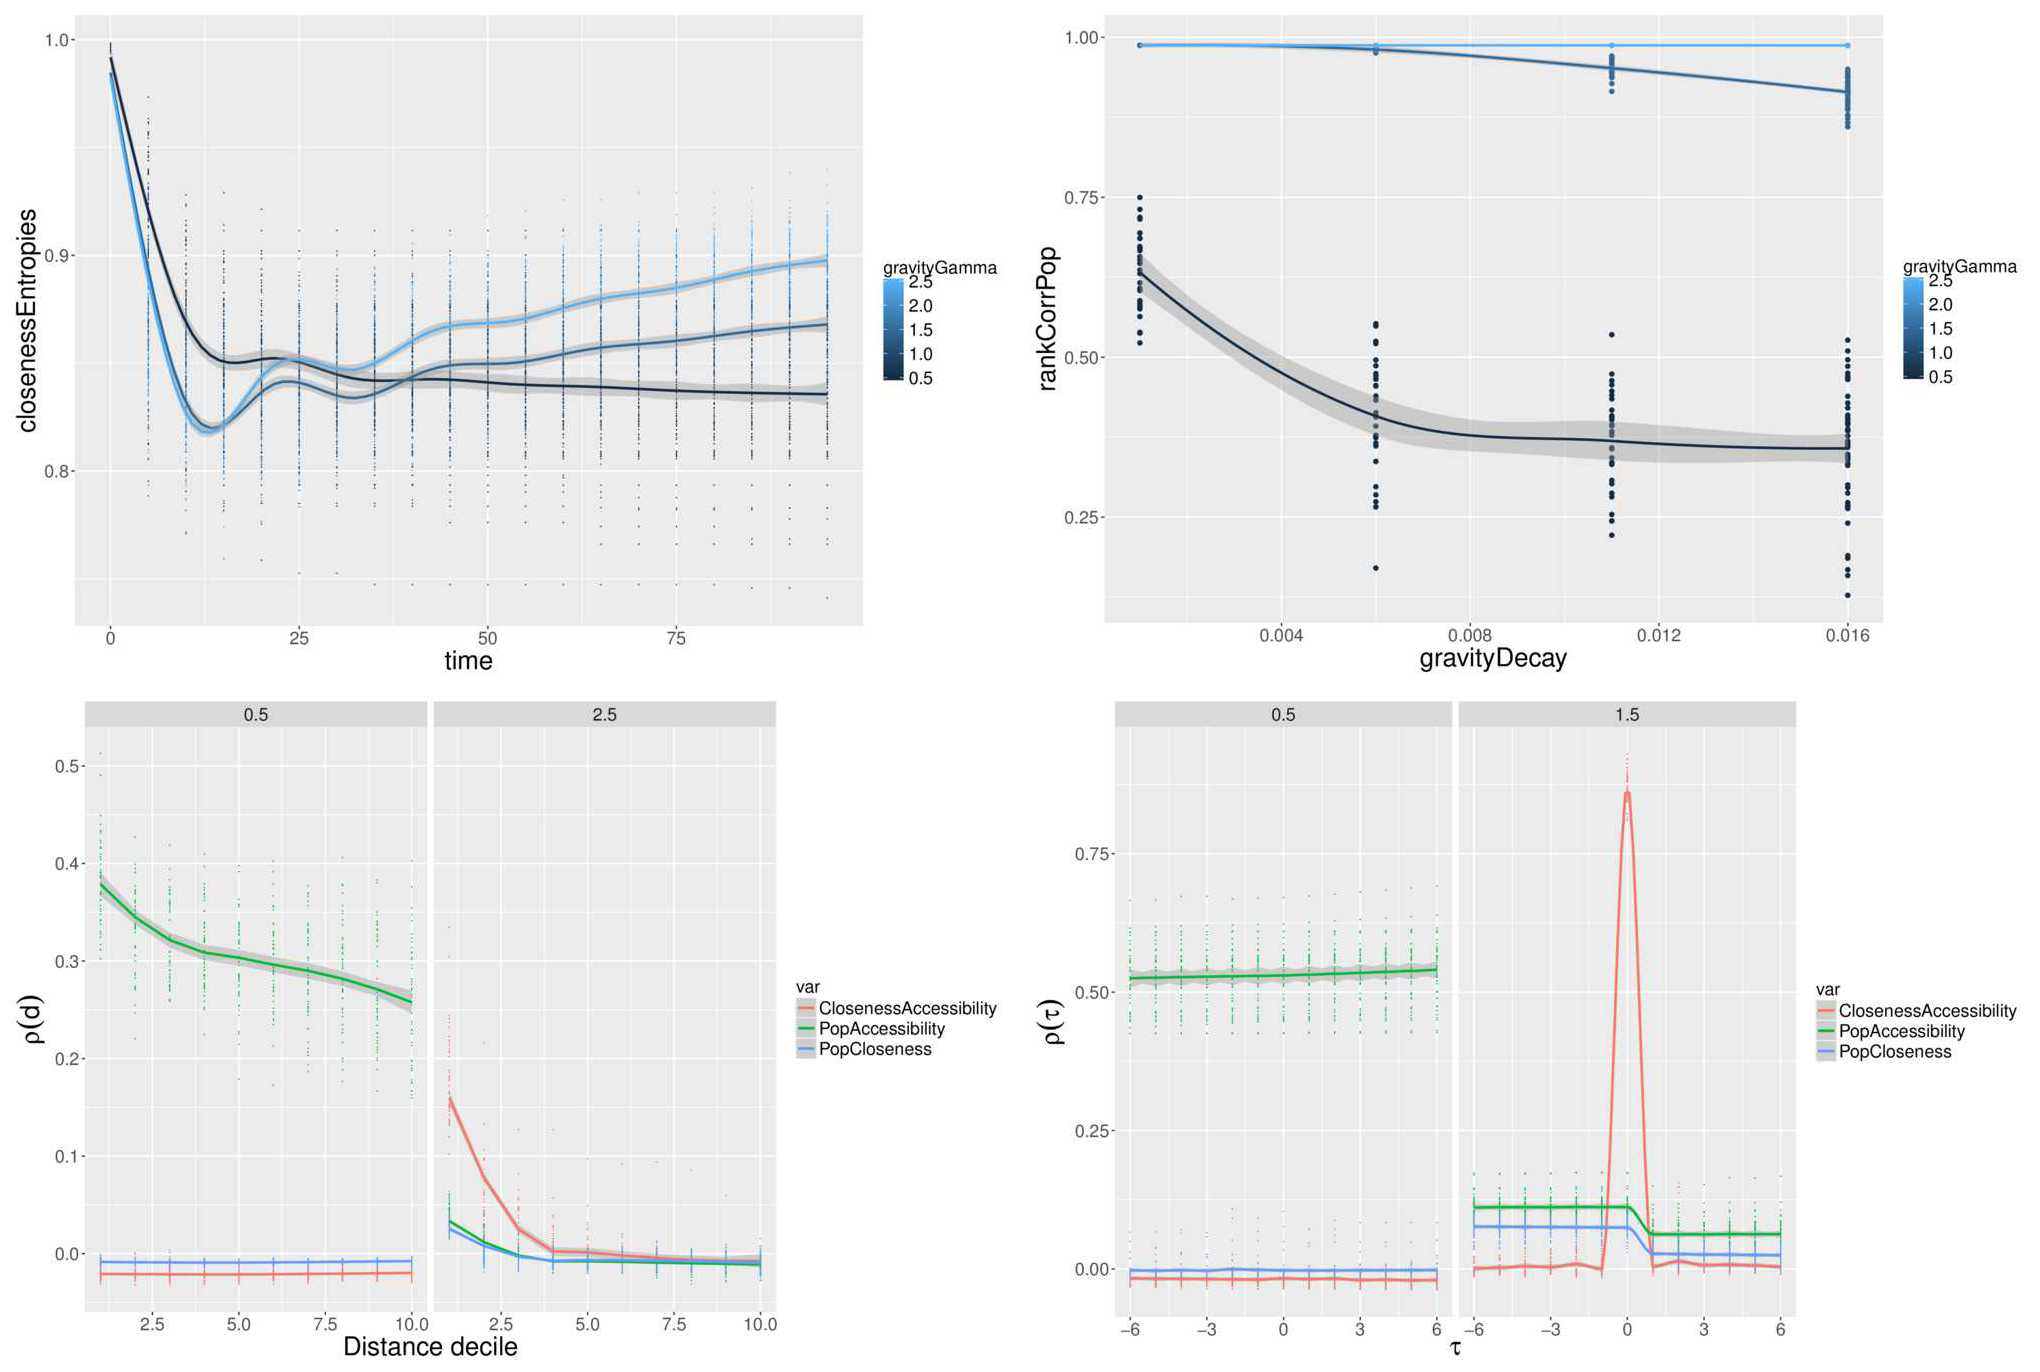
\includegraphics[width=\linewidth]{Figures/Final/6-1-3-fig-macrocoevolexplo-behavior.jpg}
	\caption[Model Behavior][Comportement du modèle]{}{\textbf{Comportement du modèle pour la configuration spatiale $N_S=80,\alpha_S=0.5,d_S=10,n_S=30$.} \textit{(Haut Gauche)} Trajectoires temporelles de l'entropie des centralités de proximité, pour $\gamma_N = 2.5$, $v_0 = 110$, $d_G = 0.016$, $\theta_N = 11$, en fonction de $\gamma_G$ (couleur); \textit{(Haut Droite)} Corrélation de rang pour la population, en fonction de $d_G$ et de $\gamma_G$ (couleur), pour $\theta_N = 11$, $\gamma_N = 2.5$; \textit{(bas Gauche)} Corrélations en fonction de la distance, pour les couples de variables (couleur), pour $\gamma_N = 2.5$, $\theta_N = 21$, $v_0 = 10$, et pour $d_G$ (colonnes) et $\gamma_G$ (lignes) variables ; \textit{(Bas Droite)} Corrélations retardées pour les mêmes paramètres. Pour les interprétations, se référer au texte.\comment[AB]{illisible}\comment[FL]{je ne commente plus les graphiques, en attente d'une refonte}\label{fig:macrocoevolexplo:behavior}}
\end{figure}
%%%%%%%%%%%%%%%%







%\subsubsection{Discussion}{Discussion}




\stars

















